\documentclass[12pt, a4paper]{article}
\usepackage[swedish, english]{babel}
\usepackage[utf8]{inputenc}
\usepackage{amsmath}
\usepackage{amsthm} %for proof
\usepackage{amssymb}
\usepackage{lmodern}
\usepackage[T1]{fontenc}
\usepackage{units}
\usepackage{icomma}
\usepackage{color}
\usepackage{float}
%\usepackage{amsfonts} %not in use
\usepackage{cancel}
\usepackage{graphicx}
\usepackage{bbm}
\usepackage{enumerate}
\usepackage{textcomp}
\usepackage{enumitem}
\usepackage{alltt}
\usepackage{amssymb}
\usepackage{datetime}
\usepackage[top=2in, bottom=1.5in, left=1.2in, right=1.2in]{geometry}
\usepackage[font=small,labelfont=bf]{caption}
\usepackage{hyperref} \hypersetup{ colorlinks=true,linktoc=all, linkcolor=blue}

\usepackage{bm}
\usepackage{fancyhdr}
\pagestyle{fancy} 
\fancyhead{} % clear all header fields
\fancyhead[L]{\normalfont\scshape\small \selectfont Edvin Listo Zec}
\fancyhead[R]{\normalfont\scshape\small \selectfont Theorems\&Proofs, PDE}
\newcommand{\N}{\ensuremath{\mathbbm{N}}}
\newcommand{\Z}{\ensuremath{\mathbbm{Z}}}
\newcommand{\Q}{\ensuremath{\mathbbm{Q}}}
\newcommand{\R}{\ensuremath{\mathbbm{R}}}
\newcommand{\C}{\ensuremath{\mathbbm{C}}}
\newcommand{\rd}{\ensuremath{\mathrm{d}}}
\newcommand{\id}{\ensuremath{\,\rd}}
% % command below makes a bold x, v and a
% % used for vector notation.
\newcommand{\xb}{\ensuremath{\mathbf{x}}}
\newcommand{\ab}{\ensuremath{\mathbf{a}}}
\newcommand{\vb}{\ensuremath{\mathbf{v}}}


\newtheorem{theorem}{Theorem}[section]
\newtheorem{corollary}{Corollary}[theorem]
\newtheorem{lemma}[theorem]{Lemma}
\newtheorem{remark}{Remark}

%% http://en.wikibooks.org/wiki/LaTeX/Advanced_Mathematics

%% //ROBIN: ADDED CODE BELOW 2014-12-08, TO SUPPORT FOR MATLAB CODE
%% TO INPUT MATLAB CODE INPUT: \lstinputlisting[language=matlab]{source_filename.m}
\usepackage{listings}
\definecolor{mygreen}{rgb}{0,0.6,0}
\definecolor{mygray}{rgb}{0.5,0.5,0.5}
\definecolor{mymauve}{rgb}{0.58,0,0.82}

\lstset{ %
  backgroundcolor=\color{white},   % choose the background color; you must add \usepackage{color} or \usepackage{xcolor}
  basicstyle=\footnotesize,        % the size of the fonts that are used for the code
  breakatwhitespace=false,         % sets if automatic breaks should only happen at whitespace
  breaklines=true,                 % sets automatic line breaking
  captionpos=b,                    % sets the caption-position to bottom
  commentstyle=\color{mygreen},    % comment style
  deletekeywords={...},            % if you want to delete keywords from the given language
  escapeinside={\%*}{*)},          % if you want to add LaTeX within your code
  extendedchars=true,              % lets you use non-ASCII characters; for 8-bits encodings only, does not work with UTF-8
  frame=single,                    % adds a frame around the code
  keepspaces=true,                 % keeps spaces in text, useful for keeping indentation of code (possibly needs columns=flexible)
  keywordstyle=\color{blue},       % keyword style
  language=Octave,                 % the language of the code
  morekeywords={*,...},            % if you want to add more keywords to the set
  numbers=left,                    % where to put the line-numbers; possible values are (none, left, right)
  numbersep=5pt,                   % how far the line-numbers are from the code
  numberstyle=\tiny\color{mygray}, % the style that is used for the line-numbers
  rulecolor=\color{black},         % if not set, the frame-color may be changed on line-breaks within not-black text (e.g. comments (green here))
  showspaces=false,                % show spaces everywhere adding particular underscores; it overrides 'showstringspaces'
  showstringspaces=false,          % underline spaces within strings only
  showtabs=false,                  % show tabs within strings adding particular underscores
  stepnumber=2,                    % the step between two line-numbers. If it's 1, each line will be numbered
  stringstyle=\color{mymauve},     % string literal style
  tabsize=2,                       % sets default tabsize to 2 spaces
  title=\lstname                   % show the filename of files included with \lstinputlisting; also try caption instead of title
}


\title{Theorems and proofs for \\ Partial differential equations \\ TMA372}
\author{Edvin Listo Zec \\ \texttt{edvinli@student.chalmers.se}}
\date{2015}
\numberwithin{equation}{section}
\begin{document}
\maketitle
\selectlanguage{english}
\thispagestyle{empty}
\centerline{\textbf{Introduction}}
\noindent This text is written as an aid for those that are taking the course TMA372 Partial differential equations. It contains the recommended theorems and proofs for the year of 2015, taken from the lecture notes of Mohammad Asadzadeh's lectures.
\newline
 \newline
 
%\centerline{\textbf{Abstract}}
%\noindent Text
\newpage
\tableofcontents
\thispagestyle{empty}
\newpage
\setcounter{page}{1}
\section{$L_\infty$ error estimates for linear interpolation in an interval}
\begin{theorem}
If $f''\in L_\infty(a,b)$ and $q=1$ (two interpolation nodes), then there are interpolation constants $c_i$ independent of $f$ and the length of $[a,b]$ such that

\begin{enumerate}[label={(\roman*)}]
    \item $||\pi_1 f - f||_{L_{\infty}(a,b)} \leq c_i (b-a)^2 ||f''||_{L_\infty(a,b)}$
    \item $||\pi_1 f - f||_{L_\infty (a,b)}\leq c_i (b-a) ||f'||_{L_\infty (a,b)}$
    \item $|| (\pi_1 f)' - f'||_{L_\infty (a,b)}\leq c_i(b-a)|| f''||_{L_\infty (a,b)}$.
\end{enumerate}
\end{theorem}
\begin{proof}
Every linear function $p(x)$ on $[a,b]$ can be written as a linear combination of the basis functions
\begin{equation*}
\lambda_a(x) = \frac{b-x}{b-a} \quad \text{ and } \quad \lambda_b(x) = \frac{x-a}{b-a}.
\end{equation*}
In other words $p(x) = p(a)\lambda_a(x)+p(b)\lambda_b(x)$. Further, we note that
\begin{equation*}
\lambda_a(x) + \lambda_b(x) = 1 \quad \text{ and } \quad a\lambda_a(x) + b\lambda_b(x) = x.
\end{equation*}

\noindent We have that 
\begin{equation}
\label{linfun}
\pi_1 f(x) = f(a)\lambda_a(x) + f(b)\lambda_b(x)
\end{equation}
is the linear function connecting the points $(a,f(a))$ and $(b,f(b))$.

\begin{figure}[H]
\centering
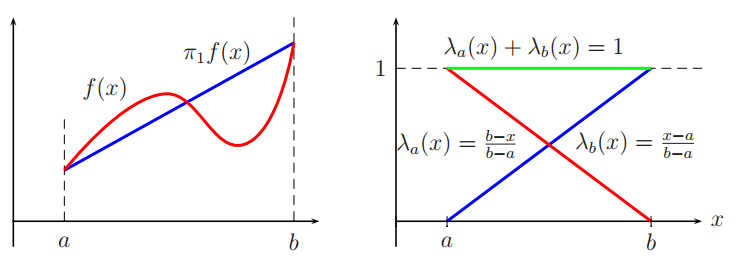
\includegraphics[scale=0.7]{th3_1_fig.png}
\caption{Linear lagrange basis functions.}
\label{sn}
\end{figure}

We now Taylor expand $f(a)$ and $f(b)$ about $x\in(a,b)$:

\begin{equation}
\label{taylor}
\left\{ \begin{array}{l}

f(a) = f(x) + (a-x)f'(x) + \frac{1}{2}(a-x)^2 f''(\eta_a), \quad \eta_a\in [a,x]\\
\\
f(b) = f(x) + (b-x)f'(x) + \frac{1}{2}(b-x)^2 f''(\eta_b), \quad \eta_b\in [x,b].

\end{array}\right.
\end{equation}

Now we insert $f(a)$ and $f(b)$ from \eqref{taylor} into $\eqref{linfun}$, and we get

\begin{equation*}
\begin{split}
\pi_1 f(x) &= f(x)[\lambda_a(x)+\lambda_b(x)] + f'(x)[(a-x)\lambda_a(x) + (b-x)\lambda_b(x)]+ \\
&+ \frac{1}{2}(a-x)^2 f''(\eta_a)\lambda_a(x)+\frac{1}{2}(b-x)^2 f''(\eta_b)\lambda_b(x)=\\
&=f(x)+\frac{1}{2}(a-x)^2f''(\eta_a)\lambda_a(x) + \frac{1}{2}(b-x)^2f''(\eta_b)\lambda_b(x).
\end{split}
\end{equation*}
Therefore
\begin{equation}
\label{diff}
|\pi_1f(x)-f(x)| = \left|\frac{1}{2}(a-x)^2f''(\eta_a)\lambda_a(x)+\frac{1}{2}(b-x)^2f''(\eta_b)\lambda_b(x)\right|.
\end{equation}
Further, we note that in the interval $x\in[a,b]$ it holds that $(a-x)^2 \leq (a-b)^2$ and $(b-x)^2\leq (a-b)^2$. Also, $\lambda_a(x)\leq 1$ and $\lambda_b(x) \leq 1, \; \forall x\in(a,b)$. Moreover, we have from the definition of the maximum norm that $|f''(\eta_a)| \leq |f''|_{L_\infty (a,b)}$ and $|f''(\eta_b)| \leq |f''|_{L_\infty (a,b)}$. This gives us that \eqref{diff} may be estimated as

\begin{equation}
|\pi_1f(x)-f(x)| \leq \frac{1}{2}(a-b)^2\cdot 1 \cdot |f''|_{L_\infty (a,b)} + \frac{1}{2}(a-b)^2\cdot 1 \cdot |f''|_{L_\infty (a,b)},
\end{equation}

and thus

\begin{equation*}
|\pi_1f(x) - f(x)|\leq (a-b)^2|f''|_{L_\infty (a,b)}\; \text{ corresponding to } c_i = 1.
\end{equation*}
The other estimates (ii) and (iii) are proved similarly.
\end{proof}

\section{BVP $\Leftrightarrow$ VF $\Leftrightarrow$ MP}
\begin{equation}
\label{bvp}
\arraycolsep=1.5pt\def\arraystretch{1.5}
\text{(BVP)}_1 \quad \left\{ \begin{array}{l}

-\big(a(x)u'(x)\big)' = f(x), \quad 0<x<1,\\
u(0)=u(1)=0.

\end{array}\right.
\end{equation}

\begin{equation}
\label{vf}
\text{(VF)}_1 \quad \int_0^1 a(x)u'(x)v'(x)\id x = \int_0^1 f(x)v(x) \id x, \; \forall v(x)\in H_0^1
\end{equation}
\\
(MP)$_1 \quad$ Find $u\in H_0^1 : F(u) \leq F(w), \; \forall w\in H_0^1$, where $F(w)$ is the total potential energy of the displacement $w(x)$:
\begin{equation}
\label{mp}
F(w) = \underbrace{\frac{1}{2}\int_0^1 a(w')^2 \id x}_\text{Internal (elastic) energy} - \underbrace{\int_0^1 fw \id x}_\text{Load potential}
\end{equation}

\begin{theorem}
The following two properties are equivalent:
\begin{enumerate}[label={(\roman*)}]
    \item $u$ satisfies \textnormal{(BVP)}$_1$
    \item $u$ is twice differentiable and satisfies \textnormal{(VF)}$_1$
\end{enumerate}
\end{theorem}

\begin{proof}
$[ \Rightarrow ]$ We assume that $a(x)$ is piecewise continuous in $(0,1)$, bounded and strictly positive for $0\leq x \leq 1$. Let $v(x)$ and $v'(x)$ be square integrable functions, i.e. $v, v' \in L_2(0,1)$. We define the following space:

\begin{equation*}
H_0^1 = \left\{ v(x) : \int_0^1 ( v(x)^2 + v'(x)^2 ) \id x < \infty, \quad v(0) = v(1) = 0 \right\}.
\end{equation*}

\noindent Now multiply (BVP)$_1$ with the test function $v(x)\in H_0^1(0,1)$ and integrate over $(0,1)$. This yields

\begin{equation*}
-\int_0^1 \big( a(x)u'(x) \big)' v(x) \id x = \int_0^1 f(x)v(x) \id x.
\end{equation*}

\noindent Integration by parts gives us

\begin{equation*}
-\big[a(x)u'(x)v(x)\big]_0^1 + \int_0^1 a(x)u'(x)v'(x) \id x = \int_0^1 f(x)v(x) \id x.
\end{equation*}
However, since $v(0)=v(1)=0$ we get (VF)$_1$:
\begin{equation*}
\int_0^1 a(x)u'(x)v(x) \id x = \int_0^1 f(x)v(x) \id x, \quad \forall v(x)\in H_0^1.
\end{equation*}
\\\\
$[\Leftarrow ]$ We start by integrating the left hand side of (VF)$_1$ by parts:
\begin{equation*}
-\int_0^1 \big( a(x)u'(x) \big)' v(x) \id x = \int_0^1 f(x)v(x) \id x, \quad \forall v(x)\in H_0^1.
\end{equation*}
This can be rewritten as:
\begin{equation}
\label{claim}
\int_0^1 \left\{ -\big ( a(x)u'(x) \big )' - f(x) \right\} v(x) \id x = 0, \quad \forall v(x)\in H_0^1.
\end{equation}
To show that $u$ satisfies (BVP)$_1$ is equivalent to claim that 
\begin{equation*}
\text{\eqref{claim}} \Rightarrow -\big (a(x)u'(x)\big )' - f(x) \equiv 0, \quad \forall x\in(0,1).
\end{equation*}
Suppose that the above claim does not hold. Then
\begin{equation*}
\exists \xi \in (0,1) : -\big ( a(\xi)u'(\xi)\big )' -f(\xi) \neq 0,
\end{equation*}
where we may assume WLOG that 
\begin{equation*}
-\big ( a(\xi)u'(\xi) \big )' - f(\xi) > 0 \;\; (\text{or } <0).
\end{equation*}
Thus, with the assumptions that $f\in C(0,1)$ and $a\in C^1(0,1)$, we have by continuity that $\exists \delta >0$, such that in a $\delta$-neighbourhood of $\xi$,
\begin{equation*}
g(x) := -\big ( a(x)u'(x) \big )' -f(x) > 0, \quad \forall x\in (\xi-\delta,\xi+\delta).
\end{equation*}
Now choose $v(x)$ from \eqref{claim} as the hat function $v^*(x)>0$ with $v^*(\xi)=1$ and the support $I_\delta := (\xi-\delta,\xi+\delta)$. Then $v^*(x)\in H_0^1$ and
\begin{equation*}
\int_0^1 \left\{ -\big ( a(x)u'(x) \big )' - f(x) \right\} v^*(x) \id x = \int_{I_\delta} \underbrace{g(x)}_{>0}\underbrace{v^*(x)}_{>0}\id x>0.
\end{equation*}
This is a contradiction of \eqref{claim}, and thus our claim holds and the proof is complete.
\end{proof}

\begin{theorem}
The following two properties are equivalent:
\begin{enumerate}[label={(\roman*)}]
    \item $u$ satisfies \textnormal{(VF)}$_1$
    \item $u$ is the solution for the minimisation problem \textnormal{(MP)}$_1$.
\end{enumerate}
In other words
    \begin{equation*}
    \int_0^1 au'v' \id x = \int_0^1 fv\id x,\; \forall v\in H_0^1 \Longleftrightarrow F(u) \leq F(w),\; \forall w \in H_0^1
    \end{equation*}
\end{theorem}
\begin{proof}
$[\Rightarrow ]$ For $w\in H_0^1$, let $v=w-u$. Then $v\in H_0^1$ since $H_0^1$ is a vector space and $u\in H_0^1$. Also
\begin{equation*}
\begin{split}
F(w) = F(u+v) &= \frac{1}{2}\int_0^1 a\big ( (u+v)' \big )^2 \id x - \int_0^1 f(u+v)\id x = \\
&=\underbrace{\frac{1}{2}\int_0^1 2au'v'\id x}_{(I)} + \underbrace{\frac{1}{2}\int_0^1 a(u')^2\id x}_{(II)} + \frac{1}{2}\int_0^1 a(v')^2\id x - \\
&- \underbrace{\int_0^1 fu \id x}_{(III)} - \underbrace{\int_0^1 fv \id x}_{(IV)}.
\end{split}
\end{equation*}
Using (VF)$_1$ we get that $(I) - (IV) = 0$. Further, by the definition of the functional F, $(II) - (III) = F(u)$. Thus
\begin{equation*}
F(w) = F(u) + \frac{1}{2}\int_0^1 a(x)(v'(x))^2\id x,
\end{equation*}
and since $a(x)>0$ we get that $F(w)\geq F(u)$ and the first implication is proven.
\\\\
$[\Leftarrow ]$ We assume that $F(u)\leq F(w)\; \forall w\in H_0^1$. Let $g_v(\epsilon) = F(u+\epsilon v)$ for an arbitrary $v\in H_0^1$. Then (MP)$_1$ gives us that $g$ (as a function of $\epsilon$) has a minimum at $\epsilon = 0$. In other words, $\frac{\id}{\id \epsilon}g_v(\epsilon) \big |_{\epsilon = 0} = 0$. We have that
\begin{equation*}
\begin{split}
g_v(\epsilon) &= F(u+\epsilon v) = \frac{1}{2}\int_0^1 a \big ( (u+\epsilon v)'\big )^2\id x - \int_0^1 f(u+\epsilon v)\id x = \\
&= \frac{1}{2}\int_0^1 \{ a(u')^2 + a\epsilon ^2 (v')^2 + 2a\epsilon u' v'\} \id x - \int_0^1 fu \id x - \epsilon \int_0^1 fv \id x,
\end{split}
\end{equation*}
and that the derivative of $g_v(\epsilon)$ is
\begin{equation*}
\frac{\id g_v(\epsilon)}{\id \epsilon} = \frac{1}{2}\int_0^1 \{ 2a\epsilon (v')^2 + 2au'v'\}\id x - \int_0^1 fv\id x.
\end{equation*}
But, $\frac{\id g_v(\epsilon)}{\id \epsilon}\big |_{\epsilon=0} = 0$, which gives
\begin{equation*}
\int_0^1 au'v'\id x - \int_0^1 fv\id x = 0,
\end{equation*}
which is our desired variational formulation (VF)$_1$. In conclusion, we can state that $F(u)\leq F(w)\; \forall w\in H_0^1 \Rightarrow \text{(VF)}_1$, which completes the proof.
\end{proof}

\section{Error estimates for BVP}
\subsubsection*{Definition}
A finite element formulation for the Dirichlet BVP \eqref{bvp} is given by: find $u_h\in V_h^{(0)}$ such that:
\begin{equation}
\label{fem}
\text{(FEM)}\quad \int_0^1 a(x)u'_h(x)v'(x)\id x = \int_0^1 f(x)v(x)\id x, \quad \forall v\in V_h^{(0)},
\end{equation}
where 
\begin{equation*}
V_h^{(0)} = \{ v : v\in C(I, P_1(I_k)), v(0)=v(1)=0 \},
\end{equation*}
$I_k = [x_{k-1}, x_{k}]$ a subinterval of $I=[0,1]$. So, $ C(I, P_1(I_k))$ denotes the set of all continuous piecewise linear functions on the partition $\tau_h = \{ 0 = x_0 < x_1 < \dots < x_M < x_{M+1} = 1\}$ of $I$.
\\\\
Note that $V_h^{(0)}$ is a finite dimensional subspace of $H_0^1$.
\\
\begin{theorem}
If $u(x)$ is a solution to the Dirichlet BVP \eqref{bvp} and $u_h(x)$ its finite element approximation defined by \eqref{fem}, then
\begin{equation}
\label{best}
||u-u_h||_E \leq ||u-v||_E, \quad \forall v(x)\in V_h^{(0)}.
\end{equation}
In other words, the finite element solution $u_h\in V_h^{(0)}$ is the best approximation in the energy norm of the solution $u$, by functions in $V_h^{(0)}$.
\end{theorem}
\begin{proof}
Take $v\in V_h^{(0)}$ arbitrarily. We have that
\begin{equation*}
\begin{split}
||u-u_h||^2_E &= \int_0^1 a(x)(u'(x)-u'_h(x))^2 \id x = \\
& = \int_0^1 a(x)\big (  u'(x)-u'_h(x) \big ) \big ( u'(x) - v'(x) + v'(x) - u'_h(x) \big )\id x = \\
&= \int_0^1 a(x)\big ( u'(x) -u'_h(x) \big )\big( u'(x) - v'(x) \big) \id x + \\
&+ \underbrace{\int_0^1 a(x) \big ( u'(x) - u'_h(x) \big ) \big ( v'(x) - u'_h(x) \big ) \id x}_{= 0 \text{ by Galerkin orthogonality since } v-u_h \in V_h^{(0)} \subset H_0^1} = \\
& = \int_0^1 a(x)^{1/2}\big ( u'(x) - u'_h(x) \big ) a(x)^{1/2}\big( u'(x) - v'(x) \big) \id x \leq \\
& \leq \left ( \int_0^1 a(x)\big ( u'(x)-u'_h(x) \big )^2\id x \right )^{1/2}\left ( \int_0^1 a(x)\big ( u'(x)-v'(x) \big )^2\id x \right )^{1/2} = \\
& = ||u-u_h||_E \cdot || u-v ||_E, \quad \forall v\in V_h^{(0)},
\end{split}
\end{equation*}
where we used Cauchy-Schwartz' inequality in the last estimate. The result is thus
\begin{equation*}
||u-u_h||_E \leq ||u-v||, \quad \forall v\in V_h^{(0)}.
\end{equation*}
\end{proof}
\begin{theorem}[A priori error estimate]
If $u$ and $u_h$ are the solutions to the \textnormal{(BVP)}$_1$ and and \textnormal{(FEM)} respectively, then there exists an interpolation constant $C_i$ depending only on $a(x)$ such that
\begin{equation*}
||u-u_h||_E \leq C_i ||hu''||_a
\end{equation*}
\end{theorem}

\begin{proof}
Since $\pi_h u(x) \in V_h^{(0)}$, we may choose $v=\pi_h u(x)$ in \eqref{best} and use an estimate from an interpolation theorem (generalised to the weighted norm $||\cdot||_a$) to get
\begin{equation*}
||u-u_h||_E \leq || u-\pi_h u ||_E = || u' - (\pi_hu)'||_a \leq C_i ||h u''||_a = C_i \left ( \int_0^1 a(x)h^2(x)u''(x)^2\id x\right )^{1/2},
\end{equation*}
which is the desired result and thus the proof is complete.
\end{proof}
\begin{remark}
The interpolation theorem is not in the weighted norm. The $a(x)$ dependence of the interpolation constant $C_i$ can be shown as follows:
\begin{equation*}
\begin{split}
||u' - (\pi_h u)'||_a &= \left ( \int_0^1 a(x)\big (u'(x)-(\pi_hu)'(x)\big)^2\id x\right)^{1/2} \leq \\
& \leq \big( \underset{x\in [0,1]}{\text{\normalfont{ max }}} a(x)^{1/2} \big )\cdot ||u'-(\pi_hu)'||_{L_2} \leq c_i \big ( \underset{x\in [0,1]}{\text{\normalfont{ max }}} a(x)^{1/2} \big )||hu''||_{L_2} = \\
&=c_i\big (\underset{x\in [0,1]}{\text{\normalfont{ max }}} a(x)^{1/2}\big ) \left (\int_0^1 h(x)^2u''(x)^2\id x\right )^{1/2} \leq \\
&\leq c_i \frac{\underset{x\in [0,1]}{\text{\normalfont{ max }}} a(x)^{1/2}}{\underset{x\in [0,1]}{\text{\normalfont{ min }}}a(x)^{1/2}}\left ( \int_0^1 a(x)h(x)^2u''(x)^2 \id x \right )^{1/2}.
\end{split}
\end{equation*}
So, we have that 
\begin{equation*}
C_i = c_i \frac{\underset{x\in [0,1]}{\text{\normalfont{ max }}}a(x)^{1/2}}{\underset{x\in [0,1]}{\text{\normalfont{ min }}}a(x)^{1/2}},
\end{equation*}
where $c_i$ is the interpolation constant from a theorem (second estimate in theorem 3.3 from the lecture notes).
\end{remark}
\begin{theorem}[A posteriori error estimate]
There is an interpolation constant $c_i$ depending only on $a(x)$ such that the error in the finite element approximation of the \textnormal{(BVP)} satisfies
\begin{equation*}
||e(x)||_E \leq c_i \left ( \int_0^1 \frac{1}{a(x)}h(x)^2R(u_h(x))^2\id x\right)^{1/2},
\end{equation*}
where $R(u_h(x)) = f + (a(x)u'_h(x))'$ is the residual and $e(x) := u(x)-u_h(x)\in H_0^1$.
\end{theorem}
\begin{proof}
We start with the definition of the energy norm:
\begin{equation*}
\begin{split}
||e(x)||^2_E &= \int_0^1 a(x)(e'(x))^2 \id x = \int_0^1 a(x)\big(u'(x)-u'_h(x)\big)e'(x) \id x = \\
& = \int_0^1 a(x)u'(x)e'(x) \id x - \int_0^1 a(x)u'_h(x)e'(x)\id x.
\end{split}
\end{equation*}
Further, we know that $e\in H_0^1$, so the variational formulation $(VF)_1$ gives
\begin{equation*}
\int_0^1 a(x)u'(x)e'(x) \id x = \int_0^1 f(x)e(x) \id x.
\end{equation*}
This gives
\begin{equation*}
||e(x)||^2_E = \int_0^1 f(x)e(x)\id x - \int_0^1 a(x)u'_h(x)e'(x)\id x.
\end{equation*}
We now add and subtract the interpolant $\pi_he(x)$ and its derivative $(\pi_he)'(x)$ to $e$ and $e'$ in the integrands, which yields
\begin{equation*}
\begin{split}
||e(x)||^2_E &= \int_0^1f(x)\big(e(x)-\pi_he(x)\big)\id x + \underbrace{\int_0^1 f(x)\pi_he(x)\id x}_{(i)} - \\
& -\int_0^1 a(x)u'_h(x)\big(e'(x) - (\pi_he)'(x)\big)\id x - \underbrace{\int_0^1 a(x)u'_h(x)(\pi_he)'(x) \id x}_{(ii)}.
\end{split}
\end{equation*}
We now have that $(i)-(ii) = 0$, since $u_h(x)$ is a solution of (FEM) and $\pi_he(x)\in V_h^{(0)}$. Thus we have
\begin{equation*}
\begin{split}
||e(x)||^2_E &= \int_0^1 f(x)\big( e(x)-\pi_he(x)\big)\id x - \int_0^1 a(x)u'_h(x)\big(e'(x)-(\pi_he)'(x)\big)\id x = \\
&= \int_0^1 f(x)\big (e(x)-\pi_h e(x)\big)  \id x - \sum_{k=1}^{M+1} \int_{x_{k-1}}^{x_k} a(x) u'_h(x)\big( e'(x)-(\pi_he)'(x)\big)\id x.
\end{split}
\end{equation*}
Further, we integrate by parts in the integrals in the sum:
\begin{equation*}
\begin{split}
& -\int_{x_{k-1}}^{x_k} a(x) u'_h(x)\big( e'(x)-(\pi_he)'(x)\big)\id x = \\
&=- \Big[ a(x)u'_h(x)\big( e(x)-\pi_he(x) \big) \Big]_{x_{k_1}}^{x_k} + \int_{x_{k-1}}^{x_k} \big (a(x)u'_h(x)\big)'\big(e(x)-\pi_he(x)\big)\id x.
\end{split}
\end{equation*}
Now we use the fact that $e(x_k) = \pi_he(x_k)$ for $k=1,2,\dots,M+1$, where $x_k$ are the interpolation nodes. This makes the boundary terms vanish and we have
\begin{equation*}
\begin{split}
-\int_{x_{k-1}}^{x_k} a(x)u'_h(x)\big(e'(x)-(\pi_he)'(x)\big ) \id x = \int_{x_{k-1}}^{x_k} \big( a(x)u'_h(x)\big)'\big(e(x)-\pi_he(x)\big)\id x.
\end{split}
\end{equation*}
Now we sum over $k$ to get
\begin{equation*}
-\int_0^1 a(x)u'_h(x)\big(e'(x)-(\pi_he)'(x)\big ) \id x = \int_0^1 \big( a(x)u'_h(x)\big)'\big(e(x)-\pi_he(x)\big)\id x,
\end{equation*}
\noindent where we interpret $\big(a(x)u'_h(x)\big)$ on each local subinterval $[x_{k-1}, x_k]$, since $u'_h$ in general is discontinuous which implies that $u''_h$ does not exist globally on $[0,1]$. Thus
\begin{equation*}
\begin{split}
||e(x)||^2_E &= \int_0^1 f(x)\big(e(x)-\pi_he(x)\big)\id x +\int_0^1 \big(a(x)u'_h(x)\big)'\big(e(x)-\pi_he(x)\big)\id x =\\
&= \int_0^1 \Big[f(x)+\big(a(x)u'_h(x)\big)'\Big]\Big[e(x)-\pi_he(x)\Big]\id x.
\end{split}
\end{equation*}
Now we let the residual error be $R(u_h(x)) = f(x)+\big(a(x)u'_h(x)\big)'$. This is a well-defined function except in in the set $\{x_k\}, k=1,\dots,M-1$ since $\big(a(x_k)u'_h(x_k)\big)'$ is not defined there. By now using Cauchy-Schwartz' inequality we get
\begin{equation*}
\begin{split}
||e(x)||^2_E &= \int_0^1 R(u_h(x))\big(e(x)-\pi_he(x)\big)\id x = \\
&= \int_0^1 \frac{1}{\sqrt{a(x)}}h(x)R(u_h(x)) \sqrt{a(x)}\left( \frac{e(x)-\pi_he(x)}{h(x)}\right)\id x \leq \\
&\leq \left( \int_0^1 \frac{1}{a(x)}h^2(x)R^2(u_h(x))\id x \right)^{1/2}\left(\int_0^1 a(x)\left(\frac{e(x)-\pi_he(x)}{h(x)}\right)^2\id x\right)^{1/2}.
\end{split}
\end{equation*}
Now, by the definition of the $L_2$-norm we get that
\begin{equation}
\label{bajs}
\left |\left| \frac{e(x)-\pi_he(x)}{h(x)} \right | \right |_a = \left( \int_0^1 a(x) \left ( \frac{e(x)-\pi_he(x)}{h(x)} \right ) ^2\id x \right ) ^{1/2}.
\end{equation}
To estimate equation \eqref{bajs} we can use an interpolation estimate for $e(x)$ in each subinterval which gives us
\begin{equation*}
\left | \left | \frac{e(x)-\pi_he(x)}{h(x)} \right | \right |_a \leq C_i||e'(x)||_a = C_i||e(x)||_E,
\end{equation*}
for a constant $C_i$ dependent on $a(x)$. Thus,
\begin{equation*}
||e(x)||^2_E \leq \left( \int_0^1 \frac{1}{a(x)}h^2(x)R^2(u_h(x))\id x\right)^{1/2} C_i||e(x)||_E,
\end{equation*}
which completes the proof.
\end{proof}
\section{Stability estimates for IVP}
Here we shall consider the following problem.
\begin{equation}
\label{DEIVP}
\left\{ \begin{array}{l}
\dot{u}(t)+a(t)u(t) = f(t), \quad 0<t\leq T\\
u(0) = u_0,
\end{array}\right.
\end{equation}
where $f(t)$ is the source term and $a(t)$ a bounded function. If $a(t)\geq0$, the problem is called parabolic, while $a(t)\geq\alpha>0$ yields a dissipative problem.

\begin{theorem}[Stability estimates]
Using the solution formula
\begin{equation}
\label{sol}
u(t) = u_0e^{-A(t)} + \int_0^t e^{-(A(t)-A(s))}f(s)\id s,
\end{equation}
where $A(s) = \int_0^t a(s) \id s$ and $e^{A(t)}$ is the integrating factor, we can derive the following stability estimates:
\\\\
(i) If $a(t)\geq \alpha > 0 $, then 
\begin{equation*}
|u(t)|\leq e^{-\alpha t}|u_0|+\frac{1}{\alpha}(1-e^{-\alpha t})\underset{0\leq s \leq t}{\text{\normalfont{ max }}} |f(s)|.
\end{equation*}
(ii) If $a(t)\geq 0$, i.e. $\alpha = 0$ (the parabolic case), then 
\begin{equation*}
|u(t)|\leq |u_0| + \int_0^t|f(s)|\id s \quad \text{or} \quad |u(t)|\leq |u_0|+||f||_{L_1(0,t)}.
\end{equation*}
\end{theorem}
\begin{proof}
We begin with \textit{(i)}. $A(t)=\int_0^t a(s)\id s$ will be an increasing function of $t$, when $a(t)\geq\alpha >0$, $A(t)\geq \alpha t$. This gives us that
\begin{equation*}
A(t)-A(s) = \int_0^t a(r) \id r - \int_0^s a(r) \id r = \int_t^s a(r) \id r \geq \alpha(t-s).
\end{equation*}
Thus we get $e^{-A(t)}\leq e^{-\alpha t}$ and $e^{-(A(t)-A(s))}\leq e^{-\alpha (t-s)}$. Now we use equation \eqref{sol} to get
\begin{equation}
\label{inte}
|u(t)|\leq |u_0|e^{-\alpha t}+\int_0^t e^{-\alpha (t-s)}|f(s)|\id s.
\end{equation}
By integrating we will get the following
\begin{equation*}
\begin{aligned}
&|u(t)|\leq e^{-\alpha t}|u_0| + \underset{0\leq s \leq t}{\text{\normalfont{ max }}} |f(s)| \left [ \frac{1}{\alpha}e^{-\alpha (t-s)}\right ]_{s=0}^{s=t}, \text{ i.e. }
\\\\
&|u(t)|\leq e^{-\alpha t}|u_0|+\frac{1}{\alpha}(1-e^{-\alpha t})\underset{0\leq s \leq t}{\text{\normalfont{ max }}} |f(s)|.
\end{aligned}
\end{equation*}
This proves \textit{(i)}.
\\\\
We go further to \textit{(ii)}. We let $\alpha=0$ in equation \eqref{inte}, so we get
\begin{equation*}
|u(t)|\leq |u_0| + \int_0^t |f(s)|\id s,
\end{equation*}
which completes the proof.
\end{proof}
\section{Lax-Milgram}
Firstly, we recall:
\begin{equation*}
(u,v) = \int_0^1 u'(x)v'(x)\id x \quad \text{and}\quad \ell(v) = \int_0^1 f(x)v(x)\id x.
\end{equation*}
Secondly, in this section we will use the following expressions.
\begin{enumerate}
\item Bilinear: $a(u,v)$ satisfies the same properties as scalar products, however it does not need to be symmetric.
\item Bounded: $|a(u,v)| \leq \beta ||u|| \; ||v||$, $\beta>0$ constant.
\item Elliptic: $a(u,v) \geq \alpha ||v||^2,$ $\alpha>0$ constant.
\end{enumerate}
\begin{theorem}[Lax-Milgram theorem]
Assuming $\ell(v)$ is a bounded, linear functional on $V$ (a Hilbert space with scalar product $(u,v)$ and norm $||u||=\sqrt{(u,u)}$) and $a(u,v)$ is bilinear bounded and elliptic in $V$, then there is a unique $u\in V$ such that
\begin{equation*}
a(u,v) = \ell(v), \quad \forall v \in V.
\end{equation*}
\end{theorem}
\begin{proof}
We begin by consider the variational formulation (VF) and the minimisation problem (MP) in abstract forms:
\begin{equation*}
\begin{split}
&\text{(V)} \qquad \text{Find } u\in \mathcal{H}_0^1 \text{ such that } (u,v)=\ell(v)\; \forall v\in \mathcal{H}_0^1 \\
&\text{(M)} \qquad \text{Find } u\in \mathcal{H}_0^1 \text{ such that } F(u) = \underset{v\in\mathcal{H}_0^1}{\text{\normalfont{ min }}} F(v), \text{ with } F(v) = \frac{1}{2}||v||^2 - \ell (v).
\end{split}
\end{equation*}
We have before proven that (V) and (M) are equivalent. We will now show that (M) has a unique solution and thus we have proven the same for (V) since they are equivalent, which in turn results in that we've proven the Lax-Milgram theorem.
\\\\
We begin by noting that $\exists$ a real number $\sigma$ such that $F(v)>\sigma$, $\forall v \in \mathcal{H}_0^1$ (otherwise it would not be possible to minimise $F$). In other words, we can write
\begin{equation*}
F(v) = \frac{1}{2}||v||^2 - \ell(v) \geq \frac{1}{2}||v||^2 - \gamma ||v||,
\end{equation*}
where $\gamma$ is the constant bounding $\ell$, i.e. $|\ell(v)|\leq\gamma ||v||$. However,
\begin{equation*}
0\leq \frac{1}{2}(||v||-\gamma)^2 = \frac{1}{2} ||v||^2-\gamma ||v|| + \frac{1}{2}\gamma^2,
\end{equation*}
thus we have
\begin{equation*}
F(v) \geq \frac{1}{2}||v||^2-\gamma ||v|| \geq -\frac{1}{2}\gamma^2.
\end{equation*}
Let now $\sigma^*$ be the largest real number $\sigma$ such that
\begin{equation}
\label{fyris}
F(v) > \sigma, \; \forall v \in \mathcal{H}_0^1.
\end{equation}
Take now a sequence of  functions $\{u_k\}_{k=0}^\infty$ such that
\begin{equation}
\label{sekv}
F(u_k) \to \sigma^*.
\end{equation}
To show that \textit{there exists a unique} solution for (V) and (M) we will use the following:
\begin{enumerate}[label=(\roman*)]
\item It is always possible to find a sequence $\{u_k\}_{k=0}^\infty$ such that $F(u_k) \to \sigma^*$ (because $\R$ is complete).
\item The parallelogram law:
\begin{equation*}
||a+b||^2 + ||a-b||^2 = 2||a||^2+2||b||^2.
\end{equation*}
\end{enumerate}
Using (ii) and the linearity of $\ell$ we get
\begin{equation*}
\begin{split}
||u_k - u_j||^2 &= 2||u_k||^2 + 2||u_j||^2 - ||u_k + u_j||^2 - 4\ell(u_k) - 4\ell(u_j) + 4\ell(u_k+u_j) = \\
&= 2||u_k||^2 - 4\ell(u_k) + 2||u_j||^2 - 4\ell(u_j) - ||u_k + u_j||^2 +4\ell(u_k + u_j) = \\
&= 4F(u_k) + 4F(u_j) - 8F\left(\frac{u_k+u_j}{2}\right),
\end{split}
\end{equation*}
where we used the definition $F(v) = \frac{1}{2}||v||^2 - \ell(v)$, with $v = u_k, v = u_j$ and $v=(u_k+u_j)/2$. Also, by the linearity of $\ell$ we got:
\begin{equation*}
-||u_k+u_j||^2 +4\ell(u_k+u_j) = -4\left|\left| \frac{u_k+u_j}{2}\right|\right|^2 +8\ell\left(\frac{u_k+u_j}{2}\right) = -8F\left(\frac{u_k+u_j}{2}\right).
\end{equation*}
Now, since $F(u_k)\to \sigma^*$ and $F(u_j)\to \sigma^*$ we have that
\begin{equation*}
||u_k+u_j||^2 \leq 4F(u_k) + 4F(u_j) - 8\sigma^* \xrightarrow[k,j \to\infty]{ } 0.
\end{equation*}
We have thus shown that $\{u_k\}_{k=0}^\infty$ is a Cauchy sequence. Since $\{u_k\} \subset \mathcal{H}_0^1$ and $\mathcal{H}_0^1$ is complete, $\{u_k\}$ is a convergent sequence. In other words, $\exists u \in \mathcal{H}_0^1 : u = \lim_{k\to\infty} u_k$. So by the continuity of $F$ we have
\begin{equation}
\label{lim}
\lim_{k\to\infty} F(u_k) = F(u).
\end{equation}
Now \eqref{sekv} and \eqref{lim} gives us that $F(u)=\sigma^*$ and by \eqref{fyris} and the definition of $\sigma^*$ we have
\begin{equation*}
F(u) < F(v), \quad \forall v\in \mathcal{H}_0^1.
\end{equation*}
Thus we have shown that there is a unique solution for (M), which means there is a unique solution for (V) since (M) $\Leftrightarrow$(V). Also, we didn't use symmetry of the scalar products, which means that we've proven the Lax-Milgram theorem with the bilinear, bounded and elliptic $a(u,v)$.
\end{proof}


\section{Error estimates for the Poisson equation}
In this section we will study the Poisson equation in higher dimensions:

\begin{equation}
\label{pois}
\left\{ \begin{array}{l}
\begin{split}
-\Delta u = f, \quad &\text{in } \Omega\subset \R^d,\; d=2,3 \\
u = 0, \quad &\text{on } \partial\Omega.
\end{split}
\end{array}\right.
\end{equation}
Here $\Omega$ is a bounded domain in $\R^d$, with polygonal boundary $\partial\Omega$.
\\\\
Further notation we are going to use is
\begin{equation*}
\tau_h = \{K : \cup K = \Omega\},
\end{equation*}
where $\tau_h$ is a triangulation of the domain $\Omega$ by the element $K$ with the maximum diagonal $h =$ max diag$(K)$. Also, we shall consider continous, piecewise linear approximations for the solution $u\in H_0^1(\Omega)$ in a finite dimensional subspace defined as:
\begin{equation*}
V_h^{(0)} = \{ v(x) : v \text{ continous, piecewise linear on } \tau_h, v=0 \text{ on } \partial\Omega \}.
\end{equation*}

\begin{theorem}[A priori error estimate for the Poisson equation]
Let $e = u - U$ be the error in the continous, piecewise linear approximation $U$ of the solution $u$ of the Poisson equation \eqref{pois}. Then
\begin{equation*}
||\nabla e|| = ||\nabla(u-U)|| \leq C||hD^2u||,
\end{equation*}
for some constant $C$, and where
\begin{equation*}
D^2u = (u^2_{xx}+2u^2_{xy}+u^2_{yy})^{1/2}
\end{equation*}
\end{theorem}
\begin{proof}
For $e= u - U$ we have $\nabla e = \nabla u - \nabla U = \nabla (u-U)$. We consider the variational formulation of the problem:
\begin{equation}
\label{ivp-vf}
\text{(VF)}\quad\quad \int_\Omega \nabla u \cdot \nabla v\id x = \int_\Omega f v \id x, \quad \forall v\in H_0^1(\Omega),
\end{equation}
and the same for the approximation $U$:
\begin{equation}
\label{aprox-vf}
\text{($V_h^{(0)}$)} \quad\quad \int_\Omega \nabla U \cdot \nabla v\id x = \int_\Omega f v \id x, \quad \forall v\in V_h^{(0)}.
\end{equation}
We now subtract equation \eqref{aprox-vf} from \eqref{ivp-vf} where we restrict $v$ to $V_h^{(0)}$, and we get the Galerkin orthogonality:
\begin{equation}
\label{galerkin}
\int_\Omega (\nabla u - \nabla U) \cdot \nabla v \id x = \int_\Omega \nabla e \cdot \nabla v \id x = 0, \quad \forall v \in V_h^{(0)}.
\end{equation}
Further, we get that
\begin{equation*}
||\nabla e||^2 = \int_\Omega \nabla e \cdot \nabla e \id x = \int_\Omega \nabla e \cdot \nabla (u-U) \id x = \int_\Omega \nabla e \cdot \nabla u \id x - \int_\Omega \nabla e \cdot \nabla U \id x.
\end{equation*}
By using the Galerkin orthogonality \eqref{galerkin}, which we can do since $U\in V_h^{(0)}$, we get that
\begin{equation*}
\int_\Omega \nabla e \cdot \nabla U \id x = 0.
\end{equation*}
Thus, we can remove the $\nabla U$ term and insert $\int_\Omega \nabla e \cdot \nabla v \id x = 0,$ $\forall v\in V_h^{(0)}$:
\begin{equation*}
||\nabla e||^2 = \int_\Omega \nabla e \cdot \nabla u \id x - \int_\Omega \nabla e \cdot \nabla v \id x = \int_\Omega \nabla e \cdot \nabla (u-v) \id x \leq ||\nabla e||\;||\nabla(u-v)||.
\end{equation*}
This means that 
\begin{equation}
\label{best1}
||\nabla (u-U)|| \leq ||\nabla (u-v)||, \quad \forall v \in V_h^{(0)}.
\end{equation}
Thus, $\nabla U$ is, in the $L_2$-norm, closer to the exact solution $\nabla u$ than any other $\nabla v$, $v\in V_h^{(0)}$. In other words, measuring in $H_0^1$-norm, the error $u-U$ is orthogonal to $V_h^{(0)}$. It is possible to show that there is an interpolant $v\in V_h^{(0)}$ such that
\begin{equation}
\label{best2}
||\nabla (u-v) ||\leq C||hD^2u||,
\end{equation}
where $h=h(x)=$diag$(K)$, $x\in K$ and $C$ is a constant independent of $h$. If we now combine equations \eqref{best1} and \eqref{best2} we get
\begin{equation*}
||\nabla e|| = ||\nabla (u-U)|| \leq C||hD^2u||,
\end{equation*}
which indicates that the error is small if $h(x)$ is sufficiently small depending on $D^2u$. And thus the proof is done.
\end{proof}

\begin{theorem}[A posteriori error estimate for the Poisson equation]
Let $u$ be the solution of the Poisson equation \eqref{pois} and $U$ its continous, piecewise linear finite element approximation. Then there is a constant $C$ independent of $u$ and $h$, such that
\begin{equation*}
||u-U||\leq C||h^2 r||,
\end{equation*}
where $r=f+\Delta_h U$ is the residual with $\Delta_h$ being the discrete Laplacian defined by
\begin{equation*}
(\Delta_h U, v) = \sum_{K\in \tau_h} (\nabla U, \nabla v)_K.
\end{equation*}
\end{theorem}

\begin{proof}
We begin by considering the dual problem
\begin{equation*}
\left\{ \begin{array}{l}
\begin{split}
-\Delta\varphi(x) = &&&e(x), \qquad\quad &&x\in\Omega \\
\varphi(x) = 0, &&&x\in\partial\Omega, &&e(x)=u(x)-U(x).
\end{split}
\end{array}\right.
\end{equation*}
Then we have $e(x) = 0$, $\forall x\in\partial\Omega$, and by using Green's formula we get that
\begin{equation*}
||e||^2 = \int_\Omega ee \id x = \int_\Omega  e(-\Delta \varphi) \id x = \int_\Omega \nabla e \cdot \nabla \varphi \id x.
\end{equation*}
By the Galerkin orthogonality and the boundary condition $\varphi(x) = 0,$ $\forall x\in\partial\Omega$, we get
\begin{equation*}
\begin{split}
||e||^2 &= \int_\Omega \nabla e \cdot \nabla \varphi \id x - \int_\Omega \nabla e \cdot \nabla v\id x = \int_\Omega \nabla e \cdot \nabla (\varphi - v) \id x = \\
&=\int_\Omega (-\Delta e) (\varphi - v)\id x \leq ||h^2 r||\; ||h^{-2}(\varphi - v)|| \leq \\
& \leq C||h^2r||\; ||\Delta \varphi|| \leq C||h^2 r|| \; ||e||,
\end{split}
\end{equation*}
where we use that $-\Delta e = -\Delta u + \Delta_h U = f +\Delta_h U = r$ is the residual and choose $v$ as an interpolant of $\varphi$. Hence, the final result becomes
\begin{equation*}
||u-U|| \leq C||h^2 r||.
\end{equation*}
\end{proof}
\section{Stability and energy estimates for the heat equation in $\R^n$}
We will consider the initial boundary value problem for the heat conduction in $R^n$:
\begin{equation}
\label{heatR}
\left\{ \begin{array}{l}
\begin{split}
&&&\dot{u}(x,t) - \Delta u(x,t) = f(x,t), \qquad &\Omega\subset\R^d,\; d=1,2,3 \;\; \text{ (DE)} \\
&&&u(x,t) = 0, &0<t<T, \text{ (BC) } \\
&&&u(x,0)=u_0(x), & x\in\Omega \text{ (IC)}
\end{split}
\end{array}\right.
\end{equation}

\begin{theorem}[Energy estimates]
Let $f\equiv 0$. Then the solution $u$ of the heat equation \eqref{heatR} satisfies the following stability estimates:
\begin{equation}
\label{ett}
\textnormal{max}\left( ||u||(t), 2\int_0^t ||\nabla u||^2(s)\id s \right ) \leq ||u_0||^2
\end{equation}
\begin{equation}
\label{sex}
||\nabla u||(t) \leq \frac{1}{\sqrt{2t}}||u_0||
\end{equation}
\begin{equation}
\label{sju}
\left( \int_0^t s||\Delta u||^2(s)\id s\right)^{1/2} \leq \frac{1}{2}||u_0||
\end{equation}
\begin{equation}
\label{åtta}
||\Delta u||(t) \leq \frac{1}{\sqrt{2}t}||u_0||
\end{equation}
\begin{equation}
\int_\epsilon^t ||\dot{u}||(s)\id s \leq \frac{1}{2}\sqrt{\ln{\frac{t}{\epsilon}}} ||u_0||
\end{equation}
\end{theorem}
\begin{proof}
Let $f\equiv 0$. To derive the first two estimates, we multiply \eqref{heatR} by $u$ and integrate over $\Omega$:
\begin{equation}
\label{udot}
\int_\Omega \dot{u}u\id x - \int_\Omega (\Delta u)u\id x = 0.
\end{equation}
We note that $\dot{u}u = \frac{1}{2}\frac{\id}{\id t} u^2$, so by using Green's formula with the Dirichlet boundary condition $u=0$ on $\partial\Omega$ we get
\begin{equation*}
-\int_\Omega (\Delta u) u \id x = -\int_{\partial\Omega} (\nabla u \cdot \mathbf{n}) u \id s + \int_\Omega \nabla u \cdot \nabla u \id x = \int_\Omega |\nabla u|^2\id x.
\end{equation*}
We can thus write equation \eqref{udot} as:
\begin{equation}
\label{equ}
\frac{1}{2}\frac{\id}{\id t}\int_\Omega u^2 \id x + \int_\Omega |\nabla u|^2 \id x = 0 \Leftrightarrow \frac{1}{2}\frac{\id}{\id t}||u||^2 + ||\nabla u ||^2 = 0,
\end{equation}
where $||\cdot||$ denotes the $L_2(\Omega)$-norm. Now we substitute $t$ with $s$ and integrate equation \eqref{equ} over $s\in(0,t)$ to get
\begin{equation*}
\frac{1}{2}\int_0^t \frac{\id}{\id s}||u||^2(s)\id s + \int_0^t||\nabla u||^2(s)\id s = \frac{1}{2}||u||^2(t)-\frac{1}{2}||u||^2(0)+\int_0^t||\nabla u||^2\id s = 0.
\end{equation*}
Now by inserting $u(0)=u_0$ we have
\begin{equation*}
||u||^2(t)+2\int_0^t||\nabla u||(s) \id s = ||u_0||^2.
\end{equation*}
Thus we have the first two estimates:
\begin{equation*}
||u||(t)\leq ||u_0||, \quad \text{ and } \quad \int_0^t ||\nabla u||^2(s) \id s \leq \frac{1}{2}||u_0||^2.
\end{equation*}
To derive estimates \eqref{sex} and \eqref{sju} we now instead multiply $\dot{u}-\Delta u = 0$ with $-t\Delta u$ and integrate over $\Omega$ to get
\begin{equation}
\label{ton}
-t\int_\Omega \dot{u}\Delta u \id x + t \int_\Omega (\Delta u)^2 \id x = 0.
\end{equation}
Green's formula ($u=0$ on $\partial\Omega \Rightarrow \dot{u} = 0$ on $\partial\Omega$) gives us that
\begin{equation*}
\int_\Omega \dot{u}\Delta u \id x = - \int_\Omega \nabla \dot{u} \cdot \nabla u \id x = - \frac{1}{2}\frac{\id}{\id t}||\nabla u||^2,
\end{equation*}
so equation \eqref{ton} can be rewritten as
\begin{equation*}
t\frac{1}{2}\frac{\id}{\id t}||\nabla u||^2 + t ||\Delta u||^2 = 0.
\end{equation*}
Further, the above equation can be rewritten using the relation $t\frac{\id}{\id t}||\nabla u||^2 = \frac{\id}{\id t}(t||\nabla u||^2) - ||\nabla u||^2$:
\begin{equation*}
\frac{\id}{\id t}\left(t ||\nabla u||^2\right) + 2t||\Delta u||^2 = ||\nabla u||^2.
\end{equation*}
Again, we substitute $t$ with $s$ and integrate over $(0,t)$:
\begin{equation*}
\int_0^t \frac{\id}{\id s}\left ( s||\nabla u||^2\right ) \id s + \int_0^t 2s||\Delta u||^2 (s) \id s = \int_0^t ||\nabla u||^2(s) \id s.
\end{equation*}
Now, from equation \eqref{ett} we have that the last equality is estimated as
\begin{equation*}
t||\nabla u||^2(t) + 2\int_0^t s||\Delta u||^2(s) \id s \leq \frac{1}{2}||u_0||^2.
\end{equation*}
From this we have
\begin{equation*}
||\nabla u||(t) \leq \frac{1}{\sqrt{2t}}||u_0|| \quad \text{ and } \quad \left(\int_0^t s||\Delta u||^2(s)\id s \right )^{1/2} \leq \frac{1}{2}||u_0||,
\end{equation*}
which are \eqref{sex} and \eqref{sju}. The estimate \eqref{åtta} is proved analogously.
\\\\
To prove the last estimate we use $\dot{u} = \Delta u$ and \eqref{åtta} to write
\begin{equation*}
\begin{split}
\int_\epsilon^t ||\dot{u}||(s) \id s\ &= \int_\epsilon^t ||\Delta u||(s) \id s = \int_\epsilon^t \frac{1}{\sqrt{s}}\sqrt{s}||\Delta u||(s)\id s \leq \\
&\leq \left ( \int_\epsilon^t \frac{1}{s} \id s\right )^{1/2}\left ( \int_\epsilon^t s ||\Delta u||^2(s) \id s \right )^{1/2} \leq \frac{1}{2}\sqrt{\ln{\frac{t}{\epsilon}}}||u_0||.
\end{split}
\end{equation*}
In the last two inequalities we used Cauchy-Schwartz  inequality and \eqref{sju}, respectively. Thus all estimates are proven, and the proof is done.
\end{proof}
\end{document}